%------------------------------------------------
% cuseip_poster.tex
\documentclass{a0poster}

% date format
\def\today{\number\day/\number\month/\number\year}

% layout
\usepackage[margin=5em]{geometry}
\setlength{\parindent}{0ex}
\setlength{\parskip}{1.5ex}

% language
\usepackage[cy]{cambi}
\usepackage{lipsum}

% packages
\usepackage{tikz}
\usepackage{framed}
\usepackage{paracol}
\usepackage{graphicx}
\graphicspath{{./figures/}}

% boxes
\usepackage[framemethod=tikz]{mdframed}
\mdfsetup{innerleftmargin=1em, innertopmargin=1em, innerrightmargin=1em, innerbottommargin=1em}
\mdfsetup{skipabove=1em,roundcorner=1em}
\newmdenv[linecolor=black]{pbox}

% fonts
%\usepackage{helvet}
\renewcommand\familydefault{\sfdefault}

%\columnratio{0.45,0.45}
%\setcolumnwidth{0.45\textwidth,0.45\textwidth}[0.1\textwidth]

% in-built Latex commands for columns
\setlength\columnsep{0.02\textwidth}
%\setlength{\columnseprule}{1pt}

%\usepackage[table,dvipsnames]{xcolor}
\usepackage{multirow}
\usepackage{tabularx}
\newcolumntype{L}{>{\raggedright\arraybackslash}X}
\newcolumntype{C}{>{\centering\arraybackslash}X}
\newcolumntype{R}{>{\raggedleft\arraybackslash}X}
\renewcommand{\arraystretch}{1.1}
\setlength{\tabcolsep}{10ex}

% keep roman logo
\let\oldLaTeX=\LaTeX
\def\LaTeX{\rmfamily\oldLaTeX\ \normalfont}

\usepackage{fancyvrb}

% colours
\usepackage{xcolor}
\definecolor{deepblue}{rgb}{0,0,0.5}
\definecolor{deepred}{rgb}{0.6,0,0}
\definecolor{deepgreen}{rgb}{0,0.6,0}
\newcommand{\red}[1]{\color{red}#1\color{black}}
\newcommand{\blue}[1]{\color{blue}#1\color{black}}
\newcommand{\green}[1]{\color{deepgreen}#1\color{black}}


%------------------------------------------------
\begin{document}
\LARGE
%------------------------------------------------

%------------------------------------------------
% HEADING
%------------------------------------------------
\setlength{\tabcolsep}{4pt}
\begin{tabularx}{\textwidth}{p{0.1\textwidth}p{0.25\textwidth}Cp{0.25\textwidth}p{0.1\textwidth}}
\parbox[c]{\linewidth}{
\includegraphics[scale=1.4]{logo.jpg}}
&
\Huge School of Mathematics\par Summer 2017
&
\VeryHuge Rebecca James \par
& 
\raggedleft
\Huge Yr Ysgol Fathemateg\par Haf 2017
&
\parbox{\linewidth}{\raggedleft
\includegraphics[scale=1.4]{logo.jpg}}
\end{tabularx}

\vspace*{2ex}
%------------------------------------------------
% TITLE
%------------------------------------------------
\begin{paracol}{2}
\centering
\veryHuge 
Language Tools for Mathematics \\[2ex]
\switchcolumn
Celfi Iaith ar gyfer Mathemateg \\[2ex]
\end{paracol}

\begin{paracol}{3}

%------------------------------------------------
% ENGLISH TEXT
%------------------------------------------------
\begin{pbox}
\textbf{\LARGE Motivation}
\Large

Writing mathematics requires specific fonts and layouts.

\LaTeX is the standard typesetting system for mathematics.

\smallskip
\setlength{\tabcolsep}{1ex}
\begin{tabular}{lp{0.5\linewidth}}
\textbf{structure} &
\verb:\title, \chapter, \section, ...: \\
\textbf{symbols} &
\verb+\alpha, \pi, \sum, \int, ...+ \\
\textbf{styles} &
\verb+\bold, \italic, ...+ \\
\textbf{mathematics} &
\verb+\equation, \theorem, ...+ \\
\textbf{references} &
\verb+\label, \ref, \cite, ...+ \\
\end{tabular}
\smallskip

There is no built-in support for \textbf{bilingual documents}.

In this project we have developed a \LaTeX package which defines commands for marking text from different languages, so that different language versions of the same document can be typeset. The package can be used by including the following line in the document preamble.

\color{deepgreen}\verb+\usepackage{culang}+\color{black}
\end{pbox}

% en screenshot 
\begin{mdframed}
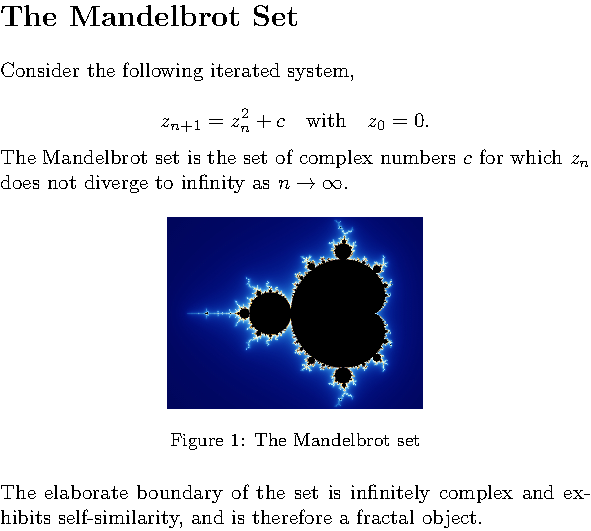
\includegraphics[width=\linewidth]{mandelbrot_en}
\end{mdframed}

\switchcolumn

%------------------------------------------------
% LATEX SOURCE CODE (VERBATIM)
%------------------------------------------------
\Large

\begin{pbox}
\begin{Verbatim}[commandchars=*\(\)]
\documentclass{article}
*green(\usepackage{culang})

\begin{document}
\title{*blue(\en) The Mandelbrot Set *red(\cy) Set Mandelbrot}
\maketitle

*blue(\en) Consider the following iterated system,
*red(\cy) Ystyriwch y system ailadroddol ganlynol,

\begin{equation}
z_{n+1} = z_n^2 + c \text{*blue(\en) with*red(\cy) gyda} z_0 = 0.
\end{equation}

*blue(\eng){The Mandelbrot set is the set of complex numbers 
$c$ for which $z_n$ does not diverge to infinity 
as $n\to\infty$.}

*red(\cym){Set Mandelbrot yw'r set o rifau cymhlyg $c$ sydd
fel nad ydyw $z_n$ yn dargyfeirio at anfeidredd 
pan mae $n\to\infty$.}

\begin{figure}
\centering
\includegraphics[scale=0.2]{mandelbrot}
\caption{*blue(\en) The Mandelbrot set*red(\cy) Set Mandelbrot}
\end{figure}

*blue(\en) The elaborate boundary of the set is infinitely 
complex and exhibits self-similarity, and is 
therefore a fractal object.

*red(\cy) Mae ffin goeth y set yn anfeidrol gymhleth ac yn 
dangos hunan-guflunedd, ac mae felly yn 
wrthrych ffractal.

\end{document}
\end{Verbatim}
\vspace*{2ex}
\end{pbox}
% end latex source

\switchcolumn

%------------------------------------------------
% CYMRAEG TEXT
%------------------------------------------------
\begin{pbox}
\textbf{\LARGE Cymhelliant}
\Large

Mae angen ffontiau a dyluniadau penodol i ysgrifennu mathemateg.

\LaTeX yw'r system safonol ar gyfer teiposod mathemateg.

\smallskip
\setlength{\tabcolsep}{1ex}
\begin{tabular}{lp{0.5\linewidth}}
\textbf{strwythyr} &
\verb:\title, \chapter, \section, ...: \\
\textbf{symbolau} &
\verb+\alpha, \pi, \sum, \int, ...+ \\
\textbf{arddulliau} &
\verb+\bold, \italic, ...+ \\
\textbf{mathemateg} &
\verb+\equation, \theorem, ...+ \\
\textbf{cyfeiriadau} &
\verb+\label, \ref, \cite, ...+ \\
\end{tabular}
\smallskip

Does dim cefnogaeth gynhenid ar gyfer \textbf{dogfennau ddwyieithog}.

Rydym wedi datblygu pecyn \LaTeX sydd yn diffinio gorchmynion ar gyfer clustnodi testun mewn ieithoedd gwahanol, fel gellir teiposod fersiynnau o'r ddogfen mewn gwahanol ieithoedd. Gellir defnyddio'r pecyn drwy gynnwys y linell ganlynol yn rhaglith y ddogfen.

\color{deepgreen}\verb+\usepackage{culang}+\color{black}
\end{pbox}

\begin{mdframed}
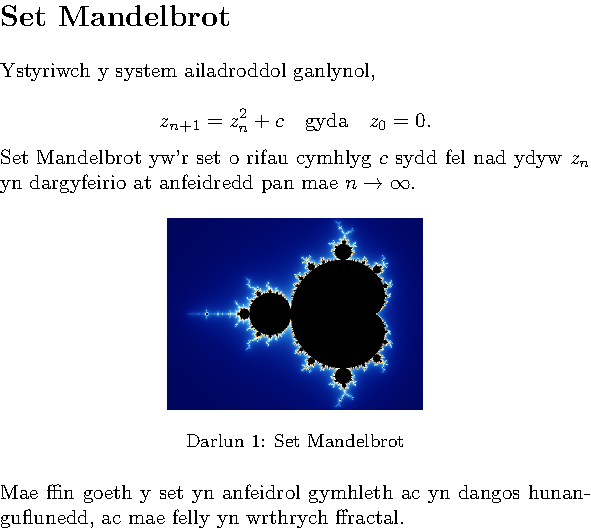
\includegraphics[width=\linewidth]{mandelbrot_cy}
\end{mdframed}
\end{paracol}

\vfill
\large
\begin{tabularx}{\linewidth}{ll>{\raggedleft\bfseries\arraybackslash}X}
\textbf{Acknowledgement}\quad\mbox{} 
& 
I would like to thank my supervisors Dr D Evans and Dr D McConnell and also the Cardiff University Centre for Education Innovation for their support in carrying out this project. 
&
Rebecca James \\
\textbf{Cydnabyddiaeth} 
& 
Hoffwn ddiolch i fy ngoruwchwylwyr Dr D Evans a Dr D McConnell ac hefyd i Ganolfan Arloesedd Dysgu Prifysgol Caerdydd am eu cefnogaeth i gyflawni'r project yma. 
&
\texttt{JamesRM5@caerdydd.ac.uk}\\
\end{tabularx}
%\end{pbox}

%------------------------------------------------
\end{document}
%------------------------------------------------

